\documentclass[a4paper,11pt,oneside,openany]{memoir}
\usepackage{fontspec}
\usepackage{amsmath} % a pretty standard package to enlarge your inventory of symbols
\usepackage{amssymb} % another common package for symbols
\usepackage[hidelinks]{hyperref} % enables hyperlinks in your document (no worries -- they show up only on the screen. When you print a hard copy, the colored boxes aren't there)
\usepackage{url} % helps typeset URLs properly, typically with the command \url
\usepackage[margin=.75in]{geometry} % page layout
\usepackage{tikz}
\usepackage{tikz-qtree}
\usepackage{wrapfig}
\usepackage{booktabs} % creates beautiful and professional tables
\usepackage{multirow}
\usepackage{textcomp}
\usepackage{expex}
\usepackage{tablefootnote}
\usepackage[calc,english]{datetime2}
\usepackage{bookmark}
\usepackage{blindtext}
\usepackage{phonrule}

\setmainfont{Charis SIL}[CharacterVariant=43:1]

%\setlength{\parindent}{2em}
\setlength{\parskip}{1ex}
%\linespread{1.1}
%---generic symbols---%
\newcommand{\dao}{$\to$}
\newcommand{\nm}{\symbol{"2205}}
\newcommand{\ra}{\textgreater}
\newcommand{\ipkt}{·}
\newcommand{\til}{\textasciitilde}
\newcommand{\langbr}{⟨}
\newcommand{\rangbr}{⟩}

\newcommand{\ortho}[1]{$\langle$#1$\rangle$}
\newcommand{\bripa}[1]{[#1]}
\newcommand{\phipa}[1]{/#1/}
\newcommand{\eng}[1]{`#1'}
\newcommand{\gob}[1]{``#1''}
%\newcommand{\ortho2}[1]{⟨#1⟩}

%---LANG'S ORTHO---%
\newcommand{\vt}{ť}
\newcommand{\vd}{ď}
\newcommand{\vc}{č}
\newcommand{\vz}{ž}
\newcommand{\vs}{š}
\newcommand{\vr}{ř}
\newcommand{\vl}{ľ}
\newcommand{\vn}{ň}
\newcommand{\vT}{Ť}
\newcommand{\vD}{Ď}
\newcommand{\vC}{Č}
\newcommand{\vZ}{Ž}
\newcommand{\vS}{Š}
\newcommand{\vR}{Ř}
\newcommand{\vL}{Ľ}
\newcommand{\vN}{Ň}
\newcommand{\Engma}{Ŋ}
\newcommand{\dbl}{ⱡ}
\newcommand{\dbL}{Ⱡ}
\newcommand{\lam}{λ}
\newcommand{\lambar}{ƛ}

%---IPA---%
%consonants
\newcommand{\bilaf}{ɸ}
\newcommand{\bilav}{β}
\newcommand{\labrox}{ʋ}
\newcommand{\latfric}{ɬ}
\newcommand{\latfrivoic}{ɮ}
\newcommand{\alvr}{ɹ}
\newcommand{\alvrap}{ɾ}
\newcommand{\alvlap}{ɺ}
\newcommand{\esh}{ʃ}
\newcommand{\ezh}{ʒ}
\newcommand{\alvpalesh}{ɕ}
\newcommand{\alvpalezh}{ʑ}
\newcommand{\paljstop}{ɟ}
\newcommand{\paljfric}{ʝ}
\newcommand{\egna}{ɲ}
\newcommand{\retesh}{ʂ}
\newcommand{\retezh}{ʐ}
\newcommand{\retna}{ɳ}
\newcommand{\egh}{ɣ}
\newcommand{\engma}{ŋ}
\newcommand{\vell}{ʟ}
\newcommand{\velr}{ʁ}
\newcommand{\glotstop}{ʔ}
%vowels
\newcommand{\frno}{ø}
\newcommand{\bari}{ɨ}
\newcommand{\unru}{ɯ}
\newcommand{\unro}{ɤ}
\newcommand{\eps}{ɛ}
\newcommand{\oeps}{œ}
\newcommand{\sche}{ɘ}
\newcommand{\schwa}{ə}
\newcommand{\centruh}{ɜ}
\newcommand{\opno}{ɔ}
\newcommand{\aesh}{æ}
\newcommand{\oesh}{ɶ}
\newcommand{\centra}{ɐ}
\newcommand{\ahoh}{ɒ}
%diacritics and modifiers
\newcommand{\asp}{ʰ}
\newcommand{\lab}{ʷ}
\newcommand{\pal}{ʲ}
\newcommand{\jekt}{ʼ}
\newcommand{\rhot}{˞}
\newcommand{\sylb}{̩}
\newcommand{\vless}{̥}
\newcommand{\upvless}{̊}
\newcommand{\retr}{̠}
\newcommand{\lamino}{̻}
\newcommand{\apico}{̺}
\newcommand{\lowap}{̞}
\newcommand{\prstr}{ˈ}
\newcommand{\scstr}{ˌ}
\newcommand{\tiebar}{͡}

\lingset{glstyle=nlevel,numoffset=3em,textoffset=1.5em,exskip=.75ex,belowglpreambleskip=.25ex,aboveglftskip=.25ex}

\DTMnewdatestyle{eurodate}{%
    \renewcommand{\DTMdisplaydate}[4]{%
        \number##3.\nobreakspace%           day
        \DTMmonthname{##2}\nobreakspace%    month
        \number##1%                         year
    }%
    \renewcommand{\DTMDisplaydate}{\DTMdisplaydate}%
}

\DTMsetdatestyle{eurodate}

\newlength{\drop}% for my convenience
\newcommand*{\titleP}{\begingroup%
%\FSfont{5bo} % FontSite Bergamo (Bembo)
\drop = 0.12\textheight
\vspace*{\drop}
\hspace*{0.3\textwidth}
{\HUGE\sc Geobo\engma}\\[\baselineskip]
\hspace*{0.33\textwidth}
{\huge A Grammar}\par
\vspace*{3\drop}
{\large By {\sc Bethany E. Toma}}
\vfill
{\today}
\vspace*{0.5\drop}
\endgroup}

\maxsecnumdepth{subsection}

\begin{document}

\begin{titlingpage}
\titleP
%\clearpage
\end{titlingpage}
\frontmatter

\chapter{Background \& Motivation}

Geobo{\engma} is a conlang spoken by a race of goblins in my as-of-yet-unnamed conworld. As goblins are sort of an underclass, their language will always be in a semi-precarious diglossic situation, and in the future I hope to add some fun sociolinguistics and diachronics based on interactions with the other languages from this conworld.

This language is intended to have some deliberately weird elements yet still retain a veneer of quasi-naturalism---while naturalism is definitely a concern, it can be discarded for the sake of trying out something fun.

\clearpage
\tableofcontents

\chapter{World \& Culture}

To-do.

\mainmatter

\chapter{Phonology}

\section{Phoneme Inventory}

With an inventory of 29 consonants and 6-7 vowels (depending on analysis, Geobo\engma's inventory isn't particularly noteworthy in its size. The distribution of its phonemes, however, could be seen as a bit abnormal, particularly when it comes to the vowels.

\subsection{Consonant Inventory}

\begin{table}[h]
    \centering
\begin{tabular}{@{}rcccccccc@{}}
\toprule
\multicolumn{1}{c}{} & \multirow{2}{*}{Bilabial} & \multicolumn{2}{c}{Laminodental} & \multicolumn{2}{c}{Apical} & \multirow{2}{*}{Palatal} & \multirow{2}{*}{Velar} & \multirow{2}{*}{Glottal} \\
\multicolumn{1}{l}{} &  & Non-Sibilant & Sibilant & Non-Sibilant & Sibilant &  &  &  \\ \midrule
Nasal & m & n\lamino &  & n\apico &  & \egna & \engma &  \\
Stop & p b & t{\lamino} d\lamino & {t\tiebar s\lamino} {d\tiebar z\lamino} &  t{\apico} d\apico & {t\tiebar s\apico} {d\tiebar z\apico}  & c\tiebar ç \paljstop\tiebar\paljfric & k g & \glotstop \\
Fricative &  & \latfric\lamino & s\lamino & \latfric\apico & s\apico & ç &  &  \\
Approximant &  & {\alvr\lamino} {l\lamino} &  & {\alvr\apico} {l\apico} &  &  &  &  \\ \bottomrule
\end{tabular}
    \caption{Consonants}
    \label{tab:consonants}
\end{table}

Geobo\engma's consonant inventory is on the larger size, and distinguishes between six places of articulation. Notably, there is a distinction between laminodental and apicoalveolar coronal consonants, as well as a distinction between sibilant and non-sibilant coronal stops/affricates and fricatives. The result remains, however, a very balanced inventory, and Geobo\engma{} is thus not notable for its consonants.

It should be noted that Geobo\engma{} orthography possesses distinct symbols for \bripa{t\tiebar\latfric\lamino}, \bripa{t\tiebar\latfric\apico}, and \bripa{x}. However, due to their distributions, these are generally not analyzed as distinct phonemes but rather as allophonic realizations of other phonemes/clusters of phonemes. This is elaborated on in Section \ref{sec:allophony}. 

\subsection{Vowel Inventory}

\begin{table}[h]
    \centering
\begin{tabular}{@{}rccc@{}}
\toprule
 & \multicolumn{1}{c}{\multirow{2}{*}{Front}} & \multicolumn{2}{c}{Back} \\
 & \multicolumn{1}{c}{} & \multicolumn{1}{c}{Unrounded} & \multicolumn{1}{c}{Rounded} \\ \midrule
High & i & \unru & u \\
Mid-High & e & \unro & o \\ 
 & \multicolumn{3}{c}{\nm{} or \schwa} \\ \bottomrule
\end{tabular}
    \caption{Vowels}
    \label{tab:vowels}
\end{table}

Geobo\engma's vowel inventory is where it is particularly strange. While its size is fairly average, at six or seven vowels, their distribution is strikingly abnormal, with no low vowels whatsoever and six at mid-high or higher. If presented with vowels lower than the canonical six, Goblins will tend to analyze them as though they were mid-high vowels of equivalent front- and roundedness. 

The existence of a seventh vowel, typically analyzed as \phipa{\schwa}, is fairly contentious. If this consonant exists, it only surfaces on a phonetic level in a very small subset of phonological contexts and is otherwise realized as syllabification\footnote{Though the term `syllabification' is itself a bit of a generalization, since this is realized in various ways depending on the consonant in question.} of the following consonant. 
Many argue that these syllables are better analyzed as vowelless, with \bripa{\schwa} being epenthetic when it occurs. If this is the case, Geobo\engma{} could be said to have no vowels lower than mid-high whatsoever. Geobo\engma{} orthography, however, uses seven-vowel analysis and writes \phipa{\schwa} as \ortho{a}.

%The utter lack of phonemically open vowels in Geobo{\engma} could be considered strange. Geobo{\engma} does historically possess a phonemic \phipa{a}; however, whether it can be considered a distinct phoneme in the current language is not clear, as it does occur phonetically in any position in which it contrasts with \phipa{\unro}. One could analyze Geobo{\engma} as possessing an \phipa{a} which does not appear phonetically but causes a following sonorant or continuant to serve as the syllabic nucleus of the relevant syllable. Under this analysis, \phipa{a} has merged with \phipa{\unro} when not followed by a sonorant or continuant, as its realizations \bripa{a\til\centra\til\centruh} do not meaningfully contrast with any of \phipa{\unro}'s realizations and tend to be interpreted as \phipa{\unro} by speakers.

\section{Syllable Structure}

There are two competing analyses of Geobo\engma{} syllable structure, which depend upon one's analysis of so-called vowelless syllables. One analysis posits the widespread permissability of vowelless syllables, in which the first consonant in the rime `takes over' as the nucleus of a vowelless syllable. Others, as previously discussed, posit the existence of a seventh seldom-realized phonemic vowel \phipa{\schwa} to avoid vowelless syllables entirely. Below we discuss both analyses and their implications.

In both analyses, the onset of a syllable in Geobo\engma{} is optional, at least on a phonemic level, and can consist of any consonant optionally preceded by a sibilant fricative (represented in this section by S) and/or followed by a sonorant or continuant. In Geobo\engma{}, sonorants and continuants (i.e., all non-stop consonants) form a natural class, indicated in this section with the symbol R whenever relevant.

\subsection{Vowelless Analysis}

\begin{wrapfigure}{r}{0.35\textwidth}
    \centering
    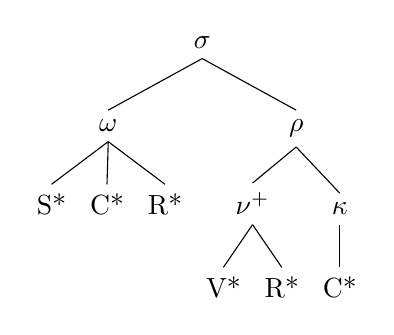
\begin{tikzpicture}
        \Tree [.$\sigma$ [.$\omega$ S* C* R* ] [.$\rho$ [.$\nu^{+}$ V* R* ] [.$\kappa$ C* ] ] ]
    \end{tikzpicture}
    \caption{Syllable Structure in Vowelless Analysis}
    \label{fig:sylb-struc-vless}
\end{wrapfigure}

In the `vowelless analysis' of Geobo\engma{} syllable structure, the nucleus of the syllable is analyzed as potentially containing both a vowel and a continuant or sonorant, but with each being optional. However, the nucleus itself is not optional and thus at least one segment, be it a consonant or vowel, must occur therein. The coda is analyzed as optional and consisting of any single consonant.

This syllable structure can also be expressed in Recursive Baerian Phonotactic Notation\footnote{Described in \url{https://llblumire.github.io/recursive-baerian-phonotactics-notation/Recursive_Baerian_Syntax_Notation.pdf}. Here we make some minor changes to the notation, moving the labels for the blocks to subscripted after the final bracket for readability. We also use $\lambda$ for word-level blocks such that $\omega$ can be freed to be used for the syllable-onset block, in keeping with traditional syllable notation.} as follows:
\begin{equation*}
\# \left[\left[\left[\:\begin{matrix}\,\begin{matrix}\textrm{S}\\\nm\end{matrix} \: \textrm{C} \: \begin{matrix}\textrm{R}\\\nm\end{matrix}\\\nm\end{matrix}\right]_\omega\left[\:\begin{matrix}\:\textrm{V} \: \begin{matrix}\textrm{R}\\\nm\end{matrix}\\\textrm{R}\end{matrix}\right]_\nu\left[\begin{matrix}\textrm{C}\\\nm\end{matrix}\right]_\kappa\:\begin{matrix}\sigma\\\nm\end{matrix}\right]_\sigma\:\right]_\lambda \#
\end{equation*}

\subsection{\phipa{\schwa} Analysis}

\begin{wrapfigure}{L}{0.35\textwidth}
    \centering
    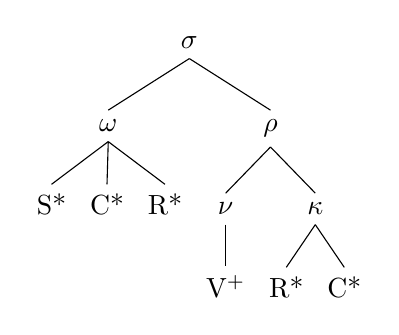
\begin{tikzpicture}
        \Tree [.$\sigma$ [.$\omega$ S* C* R* ] [.$\rho$ [.$\nu$ V$^{+}$ ] [.$\kappa$ R* C* ] ] ]
    \end{tikzpicture}
    \caption{Syllable Structure in Vowelless Analysis}
    \label{fig:sylb-struc-schwa}
\end{wrapfigure}

Among those who don't subscribe to an analysis of Geobo\engma{} as possessing vowelless syllables, the dominant approach is to analyze the syllable structure as underlyingly more symmetric and regular, such as that shown in Figure \ref{fig:sylb-struc-schwa}, with a mandatory vowel nucleus and both onset and coda allowing any consonant to cluster with a non-stop. Within this analysis, what phonetically surface as syllabic consonants are really just allophonous realizations of \phipa{\schwa} + consonant clusters. 

This structure is expressed in Baerian notation as follows:

\begin{equation*}
\# \left[\left[\left[\:\begin{matrix}\,\begin{matrix}\textrm{S}\\\nm\end{matrix} \: \textrm{C} \: \begin{matrix}\textrm{R}\\\nm\end{matrix}\\\nm\end{matrix}\right]_\omega \textrm{V}\,\: \left[\begin{matrix}\,\begin{matrix}\textrm{R}\\\nm\end{matrix} \: \textrm{C}\\\nm\end{matrix}\right]_\kappa\:\begin{matrix}\sigma\\\nm\end{matrix}\right]_\sigma\:\right]_\lambda \#
\end{equation*}

Those who champion this vowelless analysis tend to point to the relative symmetry of this structure compared to the more complicated analysis that allows for vowelless nuclei. However, those who oppose this analysis tend to point to the lack of similarity to surface forms as a point against this analysis. 

In practice, both analyses generally can capture Geobo\engma{} phenomena. In this paper, we will point out where differences between these two analyses become relevant and refer to both analyses in those cases, but by and large we will focus on the actual changes in the surface forms rather than on their theoretical syllabic structure. Where phonemic representations of relevant Geobo\engma{} words are given, a schwa will be included for clarity, but this should not be taken as being wed to the schwa analysis by any means.

\section{Phonotactics \& Allophony}\label{sec:allophony}

\subsection{Laminarity in Clusters}

Geobo\engma{} coronals can be divided into two distinct places of articulation---one lamino-dental, the other apicoalveolar. While laminarity is certainly phonemically contrastive (see, for example, \textit{k\vl e} \bripa{kl\apico e} `arm' vs. \textit{kle} \bripa{kl\lamino e} `two'), laminal and apical consonant cannot be adjacent to one another. Thus, coronals in clusters persistently assimilate in laminarity to the following consonant. 

This change is productive and does occur when compounding or inflection would result in adjacent coronals. In addition, syllabic consonants are considered adjacent to the onsets of their syllables---e.g., \textit{kla\vr} \bripa{kl\lamino\alvr\apico\sylb} would not be a legal syllable in Geobo\engma{}, and a word \phipa{kl\lamino\schwa\alvr\apico} would surface as \bripa{kl\apico\alvr\apico\sylb} and be indistinguishable from \textit{k\vl a\vr} \phipa{kl\apico\schwa\alvr\apico}. In the vowelless analysis, this is the natural extension of the restrictions on clusters, since the syllabic consonant is analyzed as being directly adjacant to the onset, and it serves as a major point in that analysis's favor. In the schwa analysis, this behavior is described as a limited form of laminal harmony. 

\setlength{\tabcolsep}{1pt}
\begin{center}
\phonc{\phonfeat[cl]{+&consonantal}}{\phonfeat[cl]{$\alpha$&distributed}}{\phold\phonfeat[cl]{+&consonantal\\$\alpha$&distributed}}
\end{center}

\subsection{Palatals and their Interactions}

When sibilant coronals are preceded by palatals, they become palatalized into alveolopalatal sibilants. 

\begin{center}
    \phonc{\phonfeat[cl]{+&consonantal\\+&anterior\\+&strident}}{\phonfeat[cl]{+&dorsal\\+&high\\-&low\\+&front\\-&back}}{\phonfeat[cl]{+&dorsal\\+&high\\-&low\\+&front\\-&back}\phold}
\end{center}

Likewise, when palatal consonants are preceded by alveolar sibilants (including alveolopalatals), they themselves become alveolopalatal sibilants.

\begin{center}
    \phonc{\phonfeat[cl]{+&consonantal\\+&coronal\\+&dorsal\\+&front}}{\phonfeat[cl]{+&anterior\\+&strident}}{\phonfeat[cl]{+&anterior\\+&strident}\phold}
\end{center}

Palatal consonants themselves are realized as velars when they precede a non-palatal consonant. Alveolopalatals are considered palatal for these purposes. 

\begin{center}
    \phonc{\phonfeat[cl]{+&consonantal\\+&coronal\\+&dorsal\\+&front}}{\phonfeat[cl]{-&coronal}}{\phold\phonfeat[cl]{+&consonantal\\$\alpha$&dorsal\\-$\alpha$&front}}
\end{center}
\noindent Unlike the other changes in this section, syllabic consonants are not considered adjacent to the last consonant in the onset. So in a word like \textit{\'sas} \phipa{ç\schwa s\lamino}, while the presence of \phipa{ç} triggers realization of \phipa{s\lamino} as \bripa{\alvpalesh}, in a word like \textit{\'sa\l} \phipa{ç\schwa\latfric\lamino} the presence of \phipa{\latfric\lamino} doesn't trigger realization of \phipa{ç} as \bripa{x}.

Palatals also condition a regressive sound change when they follow any consonantal phone that is neither labial nor glottal. Sibilant coronals become alveolopalatal in this context, while non-sibilant coronals and velar consonants are palatalized at their current place of articulation. This palatalization also occurs when these phones follow the vowel \phipa{i} as well.

\begin{center}
    \phonc{\phonfeat[cl]{+&consonantal\\-&labial\\-&constricted~glottis}}{\phonfeat[cl]{+&dorsal\\+&high\\-&low\\+&front\\-&back}}{\phold\phonfeat[cl]{+&dorsal\\+&high\\-&low\\+&front\\-&back}}
\end{center}
\noindent Palatalized coronals are all laminal, so the usual distinction between laminal and apical coronals is not maintained in environments where these phones are palatalized. This is the only aspect of these palatalization changes that is evident from the orthography, as these coronals are written using the laminal symbols---both \phipa{e\latfric\lamino ç} and \phipa{e\latfric\apico ç} would be written as \textit{e\l\'s} and realized as \bripa{e\latfric\lamino\pal ç}.

\subsection{Obstruent Voicing Assimilation}

\subsection{Nasals}

\subsection{Sibilants and Laterals}

\subsection{Changes at Vowel Hiatus}

\subsection{Onsets and Codas with Syllabic Consonants}

\subsection{Syllabic Consonants Before Onset-Less Syllables}

\subsubsection{\phipa{\glotstop} or \bripa{\glotstop}?}

\begin{enumerate}
    \item Coronal consonants persistently assimilate in laminarity to the following consonant.
    \begin{itemize}
        \item syllabic consonants included
        \item reflected in orthography
    \end{itemize}
    \item Sibilants become alveolopalatal after a palatal \& palatal obstruents become alveolopalatal after a sibilant
    \begin{itemize}
        \item syllabic consonants included
        \item \emph{not} reflected in orthography
    \end{itemize}
    \item Palatals become velar when they precede a non-palatal consonant
    \begin{itemize}
        \item syllabic consonants \emph{not} included
        \item \emph{not} reflected in orthography
    \end{itemize}
    \item Velars and non-sibilant coronals are palatalized before a palatal consonant
    \begin{itemize}
        \item syllabic consonants included
        \item \emph{not} reflected in orthography
    \end{itemize}
    \item Obstruents persistently assimilate in voice to a following obstruent. Approximants devoice before unvoiced obstruents.
    \begin{itemize}
        \item syllabic consonants included
        \item reflected in orthography \emph{sometimes} (i.e., when there is a symbol for the voiced/devoiced version of the respective sound)
    \end{itemize}
    \item Nasals assimilate in POA to a following plosive or nasal
    \begin{itemize}
        \item syllabic consonants \emph{not} included
        \item reflected in orthography
    \end{itemize}
    \item Nasals become partially-voiced non-nasal stops before a voiceless obstruent
    \begin{itemize}
        \item only applies to non-syllabic nasals
        \item only reflected in orthography when it occurs due to productive \emph{derivational} morphology, not when it occurs within a root or due to inflection
    \end{itemize}
    \item Coronal obstruents assimilate in sibilancy to a following fricative. Before a non-sibilant fricative, sibilant obstruents become lateral. Before a sibilant fricative, non-affricate stops become affricates
    \begin{itemize}
        \item syllabic consonants \emph{not} included
        \item reflected in orthography
    \end{itemize}
    \item Two of the same consonant in a row merge into a single occurrence of that consonant. Fricatives following affricates at the same place of articulation are also deleted. Partially-voiced stops absorb following voiceless stops at the same place of articulation.
    \begin{itemize}
        \item syllabic consonants included
        \item reflected in orthography
    \end{itemize}
    \item Lateral fricatives cannot be adjacent to lateral approximants
    \begin{itemize}
        \item if the approximant's placement violates the sonority hierarchy (if they are in the same syllable and it occurs before the fricative in the onset or after the fricative in the coda), the approximant is deleted
        \item if they meet at a syllable boundary, they merge and the resulting phone takes on the voicing of the latter and the manner of articulation of the former
        \item otherwise, the lateral fricative is realized as a velar non-lateral fricative
        \item reflected in orthography, but \bripa{\latfrivoic} and \bripa{l\vless} are still represented as clusters
    \end{itemize}
\end{enumerate}

\section{Orthography}
\setlength{\tabcolsep}{6pt}
\begin{center}

Coronals

\begin{tabular}{cccccccccccccccccccc}
    \ortho{t} & \ortho{\vt} & \ortho{d} & \ortho{\vd} & \ortho{c} & \ortho{\vc} & \ortho{z} & \ortho{\vz} & \ortho{s} & \ortho{\vs} & \ortho{n} & \ortho{\vn} & \ortho{r} & \ortho{\vr} & \ortho{l} & \ortho{\vl} & \ortho{\l} & \ortho{\dbl} & \ortho{\lam} & \ortho{\lambar} \\
   \bripa{t\lamino} & \bripa{t\apico} & \bripa{d\lamino} & \bripa{d\apico} & \bripa{t\tiebar s\lamino} & \bripa{t\tiebar s\apico} & \bripa{d\tiebar z\lamino} & \bripa{d\tiebar z\apico} & \bripa{s\lamino} & \bripa{s\apico} & \bripa{n\lamino} & \bripa{n\apico} & \bripa{\alvr\lamino} & \bripa{\alvr\apico} & \bripa{l\lamino} & \bripa{l\apico} & \bripa{\latfric\lamino} & \bripa{\latfric\apico} & \bripa{t\tiebar\latfric\lamino} & \bripa{t\tiebar\latfric\apico}
\end{tabular}

\vspace{1em}

Non-Coronal Consonants

\begin{tabular}{cccccccccccc}
    \ortho{p} & \ortho{b} & \ortho{m} & \ortho{\'c} & \ortho{\'z} & \ortho{\'s} & \ortho{\'n} & \ortho{k} & \ortho{g} & \ortho{\engma} & \ortho{h} & \ortho{x} \\
    \bripa{p} & \bripa{b} & \bripa{m} & \bripa{c\tiebar ç} & \bripa{\paljstop\tiebar\paljfric} & \bripa{ç} & \bripa{\egna} & \bripa{k} & \bripa{g} & \bripa{\engma} & \bripa{\glotstop} & \bripa{x}
\end{tabular}

\vspace{1em}

Vowels

\begin{tabular}{ccccccc}
    \ortho{i} & \ortho{e} & \ortho{u} & \ortho{o} & \ortho{eu} & \ortho{eo} & \ortho{a} \\
    \bripa{i} & \bripa{e} & \bripa{u} & \bripa{o} & \bripa{\unru} & \bripa{\unro} & \phipa{a} or \nm 
\end{tabular}

\end{center}

\chapter{Syntax}

\section{Animacy}

Geobo{\engma} has six noun classes. Which class a noun belongs to is based almost entirely on the lexical animacy of the noun in question. These classes form an animacy hierarchy. In Geobo{\engma}'s parent language (known as \textit{Cokizbo\engma}, lit. `finish language', to the goblins) this animacy hierarchy was fairly central to much of the morphosyntax, as it was a direct-inverse language. Modern Geobo{\engma} only shows remnants of this hierarchy in the verbal morphology, but the six third-person noun classes are still very fundamentally present in the language's morphosyntax.

\begin{table}[h]
    \centering
    \begin{tabular}{@{}rl@{}}
    \toprule
0 & 1st \& 2nd Person \\
1 & Natural Forces \\
2 & Non-Goblin Intelligent Creatures \\
3 & Goblins \\
4 & Living Animals \\
5 & Inanimate Objects \\
6 & Abstract Concepts \\
\bottomrule
\end{tabular}
    \caption{Animacy Hierarchy}
    \label{tab:anim}
\end{table}

As one of the few relics of the animacy hierarchy, there are different morphemes for verbal negation depending on the noun classes of the subject and object. If the subject is equal to or higher on the animacy hierarchy than the object, the affix \textit{-(o)keo-} is placed directly after the root. If the subject is lower on the animacy hierarchy than the object, the affix \textit{-og\'z(u)-} is used instead. 

\pex
\a
\begingl
Geob[goblin] 
te\vd[1]
bol[strike]@
-keo[-{\sc neg.dir}]@
-g[-{\sc >3.gob}]
\glft `I didn't hit a goblin.'
\endgl
\a
\begingl
Geob[goblin] 
te\vd[1]
bol[strike]@
-og\'z[-{\sc neg.inv}]@
-e\vd[-{\sc >1}]
\glft `A goblin didn't hit me.'
\endgl
\xe

\section{Verbal Morphology}

Verbs in Geobo{\engma} are suffixed with a marker for person and animacy. These markers originate from pronouns that used to be placed after the verb and thus resemble reduced forms of those pronouns. 

\begin{table}[ht]
    \centering
    \begin{tabular}{@{}rcccccccc@{}}
\toprule
 & 1st & 2nd & {\sc nt-frc} & {\sc ng-int} & {\sc gob} & {\sc animl} & {\sc inan} & {\sc abstr} \\ \midrule
Suffix\tablefootnote{When multiple suffixes are listed, the former is used when the suffix follows a non-syllabic consonant and the latter when it follows a syllabic consonant or vowel unless otherwise indicated} & \textit{-e\vd, -\vd} & \textit{-ar, -r} & \textit{-a\vn, -\vn} & \textit{-meu} & \textit{-eog, -g}\tablefootnote{If the latter suffix is used following a front vowel, that vowel is backed.} & \textit{-\vs u} & \textit{-im, -m}\tablefootnote{If the latter suffix is used following a back vowel, that vowel is fronted. Fronting of rounded vowels is allophonic and not reflected orthographically.} & \textit{-es, -s}\tablefootnote{Unlike the other listed suffixes, for the abstract noun class the latter vowelless allomorph is only used following a true vowel, and the former suffix is used following a syllabic consonant.}  \\
Pronoun & \textit{te\vd} & \textit{kar} & \textit{teu\vn} & \textit{ameu} & \textit{eog} & \textit{\vs u} & \textit{him} & \textit{es} \\
Reflexive\tablefootnote{Perhaps abnormally, reflexive forms for pronouns are used as subject pronouns rather than object pronouns} & \textit{tete\vd} & \textit{karkar} & \textit{teudteu\vn} & \textit{meum} & \textit{geog} & \textit{\vs u\vs} & \textit{himim} & \textit{ses} \\ \bottomrule
\end{tabular}
    \caption{Person/Animacy Markers}
    \label{tab:my_label}
\end{table}

These markers agree in person and animacy with the syntactic \emph{object} rather than the subject---that is, the more patientlike P argument rather than the more agentlike A argument (though the semantic roles these syntactic roles fill can obviously vary significantly depending on both the verb in question and the context). 

If both the subject and object are of the same noun class and it is thus ambiguous which entity in the sentence the agreement marking is referring to, the appropriate standalone pronoun can be placed directly after the subject. However, this is only done if the sentence would be obviously ambiguous otherwise.

\ex
\begingl
A\l k[dog]
\vs u[{\sc 3.animl}]
de{\vz}[cat]
bo\vl[strike]@
-\vs u[-{\sc >3.animl}]
\glft `The dog hit the cat.'
\endgl
\xe

Agreement with the syntactic P argument naturally leads to the question of what (if any) markings verbs take if the verb is intransitive. The simple answer is that Geobo{\engma} lacks true syntactic intransitives entirely. Rather, several different constructions are used as workarounds so that otherwise transitive Geobo{\engma} verbs can express typically-intransitive meanings.

For verbs in which the single argument does not initiate or is not actively responsible for the action of the verb, the most common solution is to use the abstract pronoun \textit{es} as a dummy subject, similar to how English would use `there' or `it' in certain types of clauses. 

\ex 
\begingl
Geob[goblin]
es[3.{\sc abstr}] 
\l emp[trip]@
-eog[-{\sc >3.gob}]
\glft `The goblin trips.' (lit., `It trips the goblin.')
\endgl
\xe

There does not have to be an unspoken agent or cause of the action described by the verb for this structure to work---the purest of statives with no actual cause can also be represented by this structure.

\ex
\begingl
Beu[berry]
es[{\sc 3.abstr}]
ka\l[red]@
-im[-{\sc >3.inan}]
\glft `The berry is red.' (lit., `It reddens the berry.')
\endgl
\xe

Many verbs, particularly those of position and motion, contrast this dummy-subject structure with another that uses reflexive pronouns. For these verbs, use of a reflexive pronoun as the subject indicates a dynamic reading, while the dummy-subject structure indicates a stative reading.

\pex
\a
\begingl
Geob[goblin]
es[{\sc 3.abstr}]
ot[sit]@
-eog[-{\sc >3.gob}]
\glft `The goblin is sitting.' (lit., `It seats the goblin.')
\endgl
\a
\begingl
Geob[goblin]
geog[{\sc 3.gob.refl}]
ot[sit]@
-eog[-{\sc >3.gob}]
\glft `The goblin sits down.' (lit., `Himself seats the goblin.')
\endgl
\xe

As evidenced by the use of the dummy-subject strategy for a verb like `to sit', it doesn't take much for an argument to be considered sufficiently un-agent-like for that strategy. Indeed, only the most prototypical agents are not captured by this strategy.

For would-be intransitive verbs where the argument explicitly represents an agent, there is yet another strategy. One can nominalize the main verb adding the suffix \textit{-stu} to the root, and then treat this nominalized verb as the object of the verb \textit{\'se} `to do, to make'.

\ex
\begingl
\vR im[run]@
-stu[-{\sc nmz}]
geob[goblin]
\'se[do]@
-s[-{\sc >3.abstr}]
\glft  `The goblin is running.' (lit., `The goblin does running.')
\endgl
\xe

For certain motion verbs, both the nominalization and reflexive strategies are both appropriate. In this case, the former allows the speaker to put the action in focus in a way that cannot be done when the action is not nominalized, as in the reflexive strategy (see section \ref{focus} for more on focus marking). In addition, the former carries connotations of duration/ongoingness, while the latter is more explicitly inchoative. Compare (\lastx) with (\nextx):

\ex
\begingl
Geob[goblin]
geog[{\sc 3.gob.refl}]
\vr im[run]@
-eog[-{\sc >3.gob}]
\glft `The goblin gets himself running.'
\endgl
\xe

The reflexive strategy is not necessarily appropriate for all would-be intransitives, however, as for many (if not most) verbs, it simply carries the expected reflexive meaning.

\ex
\begingl
Karkar[{\sc 2.refl}]
bol[strike]@
-ar[-{\sc >2}]
\glft  `You're hitting yourself.' (\emph{not} `You're getting yourself to hit things.')
\endgl
\xe

\section{Possession \& Quantification}

As Geobo{\engma} is head-marking, in a possession scenario it is the possessed noun that is inflected. A possessive affix \textit{-(a)\l-} is added to the end of the possessed noun and then followed by a suffix that agrees in person and number with its possessor. The possessor, if specified, is placed before the possessed noun.

\ex
\begingl
\vN u\'noh[elf]
meo[mother]@
-\l[-{\sc poss}]@
-meu[-{\sc 3.ngint}]
\glft  `The elf's mother'
\endgl
\xe

This syntactic structure is also used more broadly, however, for quantification. Perhaps counterintuitively, the quantified noun is treated as the possessor of the noun indicating the relevant quantity.

\ex
\begingl
\vD eo\'s[tree]
eu\'s[all]@
-a\l[-{\sc poss}]@
-m[-{\sc 3.inan}]
\glft `all of the trees' (lit., `the tree's everything')
\endgl
\xe

This is not limited to more ambiguous quantifiers---it is used for numbers as well.

\ex
\begingl
\vD eo\'s[tree]
zlic[three]@
-a\l[-{\sc poss}]@
-m[-{\sc 3.inan}]
\glft `three trees' (lit., `the tree's three')
\endgl
\xe

This use of quantifiers is one of Geobo{\engma}'s main methods of compensating for the fact that it does not mark for number whatsoever, even in pronouns. If a speaker wants to pluralize a pronoun (for instance, saying `we') that speaker can simply use the quantifier inflected for the relevant person and animacy (such as \textit{eu\'sa\dbl\vd} `all of me/us').

To quantify over verbs (i.e., to say something happened `twice' or `many times'), one must quantify over the object. This is true even if the object seems to be something unquantifiable, such as an abstract noun or nominalized verb.

\ex
\begingl
\vR im[run]@
-stu[-{\sc nmz}]
kle[two]@
-\l[-{\sc poss}]@
-es[-{\sc 3.abstr}]
te{\vd}[1]
\'se[do]@
-s[-{\sc >3.abstr}]
\glft `I ran twice.' (lit., `I did two running.')
\endgl
\xe

Distinguishing between whether a quantifier on the object semantically indicates quantification over the object or the verb is only done if context does not make it clear which is meant, but can be done using adjectives and embedding quantifiers under one another.

\pex
\a
\begingl
\vD er\engma[different]
\vs\vr eo\vd[eel]
kle[two]@
-\l[-{\sc poss}]@
-im[-{\sc 3.inan}]
te\vd[1]
\vr u[cook]@
-m[-{\sc >3.inan}]
\glft `I cooked two different eels.'
\endgl
\a
\begingl
\vS\vr eo\vd[eel]
da\'n[one]@
-a\l[-{\sc poss}]@
-m[-{\sc 3.inan}]
kle[two]@
-\l[-{\sc poss}]@
-es[-{\sc 3.abstr}]
te\vd[1]
\vr u[cook]@
-m[{\sc ->3.inan}]
\glft `I cooked one eel twice.'
\endgl
\xe

\section{Postpositions}

Postpositions follow their nouns and inflect to agree with their objects. Their endings are identical to those used for verbs.

\ex
\begingl
\vT\'ne{\vl}[stick]
\vc o[{\sc ins}]@
-m[-{\sc 3.inan}]
\glft `with a stick'
\endgl
\xe

If the postposition would only be preceded by a pronoun, it can be omitted and the inflected postposition used on its own as a whole phrase.

\ex 
\begingl 
\Engma i[away.from]@
-\vd[-1]
\vn u\'noh[elf]
meum[{\sc 3.ngint.refl}]
\vr im[run]@
-eu[-{\sc >3.ngint}]
\glft `The elf ran away from me.'
\endgl
\xe

In addition to traditional postpositions, Geobo{\engma} demonstratives are also realized as postpositions. Since postpositional phrases cannot be embedded within each other, one cannot use an explicit demonstrative with a noun that is already part of a postpositional phrase.

\pex
\a
\begingl
\Engma u{\vz}[fish]
u\vd[{\sc med}]@
-im[-{\sc 3.inan}]
kar[2]
bo\vs[eat]@
-im[-{\sc >3.inan}]
\glft `You ate that fish.'
\endgl
\a 
\begingl 
\Engma u\vz[fish]
\vc o[{\sc ins}]@
-m[-{\sc 3.inan}]
kar[2]
bol[strike]@
-e\vd[-{\sc >1}]
\glft `You hit me with a fish.'
\endgl
\a \ljudge* \textit{\Engma u{\vz} u\vd im \vc om kar bole\vd} \\
(Intended: `You hit me with that fish.')
\a \ljudge* \textit{\Engma u{\vz} \vc om u\vd im kar bole\vd} \\
(Intended: `You hit me with that fish.')
\xe

This does not otherwise change the syntactic behavior of the noun---if the argument in question is the object without the demonstrative postposition, it remains the syntactic object and verbal agreement still takes place.

\section{Ditransitives}

Geobo{\engma} is secundative, so for inherently ditransitive verbs like \textit{\'cneu} `to give', the syntactic object of the verb is the recipient. The theme can be included as a postpositional argument using the instrumental \textit{\vc o}.

\ex
\begingl
Meo[mother]@
-\l[-{\sc poss}]@
-e{\vd}[-{\sc 1}]
geob[goblin]
de{\vz}[cat]
\vc o[{\sc ins}]@
-\vs u[-{\sc 3.animl}]
\'cneu[give]@
-meu[-{\sc >3.ngint}]
\glft `The goblin gave my mother a cat.'
\endgl
\xe

Benefactive ditransitives can be derived from many verbs that are not inherently ditransitive by addition of the affix \textit{-tu-} before the agreement suffix but after the negation affix (if any).

\ex
\begingl
Meo[mother]@
-\l[-{\sc poss}]@
-ar[-2]
te{\vd}[1]
\vs\vr eo{\vd}[eel]
\vc o[{\sc ins}]@
-m[-{\sc 3.inan}] 
\vr u[cook]@
-keo[-{\sc neg.dir}]@
-tu[-{\sc ben}]@
-g[-{\sc >3.gob}]
\glft `I won't cook eel for your mother.'
\endgl
\xe

Since the theme is optional in these `ditransitives', this is also an effective way of describing an action in which the theme is unknown or unspecified, effectively serving as another argument-reduction strategy.

\ex
\begingl
Meo[mother]@
-\l[-{\sc poss}]@
-eog[-{\sc 3.gob}]
\vS krik[Skreek]
eog[{\sc 3.gob}]
de\vn\vr e[sing]@
-tu[-{\sc ben}]@
-g[-{\sc >3.gob}]
\glft `Skreek sings for his mother.'
\endgl
\xe

\section{`Adjectives'}

Strictly speaking, there is not a separate syntactic class known as `adjectives' in Geobo{\engma}. However, the equivalent of adjectives are realized by adverbs or uninflected verbs placed directly before the nouns they modify.

\pex
\a
\begingl
\'Cre\'z[alive]
\vt\'ne\vl[stick]
\glft  `Flourishing branch'
\endgl
\a 
\begingl
\vT\'nel[stick]
ban[sun]
\'cre\'z[alive]@
-im[\sc ->3.inan]
\glft `The sun made the branch flourish.'
\endgl
\xe

In more complex NPs containing possession or quantification, the location of the adjective can affect the meaning of a phrase.

\pex
\a
\begingl
\'Cre\'z[alive]
\vt\'ne{\vl}[stick]
da\'n[one]@
-a\l[-{\sc poss}]@
-m[-{\sc 3.inan}]
\glft  `One of the flourishing branches'
\endgl
\a
\begingl
\vT\'ne{\vl}[stick]
\'cre\'z[alive]
da\'n[one]@
-a\l[-{\sc poss}]@
-m[-{\sc 3.inan}]
\glft  `The flourishing one of the branches'
\endgl
\xe

As we've already seen in earlier examples, originally causative verbs can serve practically as predicative adjectives when inflected with a dummy subject

\ex
\begingl
\Engma u\vz[fish]
es[\sc 3.abstr]
nono\vn[enlarge]@
-\vs u[\sc ->3.animl]
\glft `The fish is big.' (lit., `It enlargens the fish.')
\endgl
\xe

By default, bare verbs used attributively (i.e., as adjectives in the above examples) carry the meaning characteristic to the \textit{object} of that verb---e.g., \textit{\'cre\'z} means `alive'/`flourishing' not `live-giving', \textit{uh} means `dead' not `deadly', etc. Adjectives with meanings more characteristic of the subjects of these verbs can be formed using the causative derivational prefix \textit{(o)c-} (e.g., \textit{oc\'cre\'z} `live-giving', \textit{cuh} `deadly', etc.). While this prefix technically also derives a causative verb, due to the nature of Geobo{\engma} verbs, the resulting verb is probably more often used as an attributive or predicative adjective than as a causative verb proper. 

Geobo{\engma} lacks separate comparative forms of the verb. In order to make predicative comparisons, the verb is turned into a benefactive ditranstive using the affix \textit{-tu-}. The `lesser' of the compared items then serves as the syntactic object of the verb, with the `greater' item as the optional instrumental argument, and the dummy pronoun remains the syntactic subject.

\ex 
\begingl
Reu[house]@
-\l[\sc -poss]@
-e\vd[\sc -1]
es[\sc 3.abstr]
\engma u\vz[fish] 
\vc o[\sc ins]@
-\vs u[\sc -3.animl]
nonon[enlarge]@
-tu[\sc -ben]@
-m[\sc ->3.inan]
\glft `The fish is bigger than my house.' (lit., `It enlarges the fish for my house.')
\endgl
\xe

Note that the verb still agrees with the syntactic object, so unlike in the non-comparative example, the verb agrees with the noun that is less well-described by the adjective in question. This means that in such comparisons, the standard of comparison cannot be omitted.

\section{Focus \& Word Order}\label{focus}

To the casual observer, Geobo{\engma} seems superficially OSV. While it is true that this pattern is certainly the most commonly seen in the language, the reality is more complicated. This typical ordering is actually due to the focus marking that lies at the core of Geobo{\engma} sentence structure.

In any given sentence, whichever argument is the focus is moved to a sentence-initial position. 

\ex
\begingl
A\l k[dog]
\vS krik[Skreek]
bo\vl[strike]@
-\vs u[{\sc >3.animl}]
\glft `It was the dog that Skreek hit.'
\endgl
\xe

\ex
\begingl
\vS krik[Skreek]
a\l k[dog]
bo\vl[strike]@
-\vs u[-{\sc >3.animl}]
\glft `It was Skreek who hit the dog.'
\endgl
\xe

Before this movement, the sentence is underlyingly SOV, so if a complement other than the subject or object is the focus, this is the order in which those arguments will appear.

\ex
\begingl
\vT\vn e{\vl}[stick]
\vc om[\sc ins:3.inan]
\vS krik[Skreek]
a\l k[dog]
bo\vl\vs u[strike:{\sc >3.animl}]
\glft `It was with a stick that Skreek hit the dog.'
\endgl
\xe

Only arguments can be fronted like this, so if the verb or an adjunct is the focus, the object is moved to this position in their stead. 

\pex Q: `When did Skreek hit the dog?'
\a \ljudge*
\begingl
Da\'s[yesterday]
\vS krik[Skreek]
a\l k[dog]
bo\vl\vs u[strike:{\sc >3.animl}]
\endgl
\a 
\begingl
A\l k[dog]
\vS krik[Skreek] 
da\'s[yesterday]
bo\vl\vs u[strike:{\sc >3.animl}]
\glft A: `Skreek hit the dog yesterday.'
\endgl
\xe

If the object is not in focus and would be represented with a pronoun, it can be omitted from the sentence. However, this is not the case with any other argument (i.e., subjects must always be explicitly included).

\ex
\begingl
\glpreamble A: \textit{A\l k \vS krik da\'s bo\vl\vs u.} (`Skreek hit a dog yesterday.')\\B: \textit{\'Ne\l?} (`Really?')\endpreamble
Ip[yes]
\vt\vn e{\vl}[stick]
\vc om[\sc ins:3.inan]
eog[{\sc 3.gob}]
bo\vl\vs u[strike:{\sc >3.animl}]
\glft `Yes, it was with a stick that he hit (it).'
\endgl
\xe

\section{Relative Clauses}

Geobo{\engma} relative clauses are formed via adjoined clauses. The relativized noun must be fronted in both clauses, and therefore only arguments can be relativized. The complementizer \textit{deo\l} is placed clause-initially in the relativized clause, which is then directly followed by the main clause. The argument in question can be either restated in the main clause (often with a demonstrative) or replaced with a pronoun.

\pex
\a
\begingl
Deo{\l}[{\sc c}]
oh[person]
te{\vd}[1]
\vz e\'zeog[see:{\sc >3.gob}]
\nogloss{,}
oh[person]
\'no\vd eog[{\sc dist:3.gob}]
reu[home]
eumim[go.to:{\sc >3.inan}]
\endgl
\a
\begingl
Deo{\l}[{\sc c}]
oh[person]
te{\vd}[1]
\vz e\'zeog[see:{\sc >3.gob}]
eog[{\sc 3.gob}]
reu[home]
eumim[go.to:{\sc >3.inan}]
\glft `The person who I saw went home.'
\endgl
\xe

The order of the relativized and main clause is determined by whether the relative clause is restrictive or not. In restrictive relative clauses, the relative clause precedes the main clause, while in non-restrictive relative clauses, the relative clause occurs afterwards.

\ex
\begingl
Meo\l e\vd[mother:{\sc poss:1}]
reu[home]
eumim[go.to:{\sc >3.inan}]
\nogloss{,}
deo{\l}[{\sc c}]
eog[{\sc 3.gob}]
geob[goblin]
\vz eog[\sc cop:>3.gob]
\glft `My mother, who is a goblin, went home.'
\endgl
\xe

Content clauses, in which the subordinate clause serves as an argument of the main sentence, are expressed using relative clauses modifying the dummy noun \textit{as}. Historically, \textit{as} could be roughly translated `case, situation, affair', but in the modern language it is not used outside of the formation of content clauses

\ex
\begingl
Deo{\l}[{\sc c}] 
geob[goblin]
meo\l ar[mother:{\sc poss:2}]
\vz eog[\sc cop:>3.gob]
\nogloss{,}
as[{\sc c}]
te{\vd}[1]
\vz e\'zes[see:{\sc >3.abstr}]
\glft `I saw that your mother is a goblin.' (lit., `I saw the fact that your mother is a goblin.')
\endgl
\xe

Most other subordinating conjunctions in English are approximated by using the above strategy combined with various prepositions or verbs.

\ex 
\begingl
Deo\l[\sc c]
dizd[salt]
\engma u\vz[fish]
pidim[possess:{\sc >3.inan}]
\nogloss{,}
as[\sc c]
euźdes[due\_to:{\sc 3.abstr}]
te\vd[\sc 1] 
bo\vs kem[consume:{\sc neg.dir:>3.inan}]
\glft `I didn't eat the fish because it was salty.' (lit., `Due to the fact that the fish had salt, I didn't eat it.')
\endgl
\xe 

\chapter{Semantics}

\section{TAM Particles}

Geobo{\engma} is tenseless, only specifying tense if doing so is necessary in context and doing so using temporal adverbs, which are typically placed before the verb.

\pex 
\a 
\begingl 
bostu[eat:{\sc nmz}]
te\vd[1]
da\'s[yesterday]
\'ses[do:{\sc >3.abstr}]
\glft `I ate yesterday.'
\endgl
\a 
\begingl 
bostu[eat:{\sc nmz}]
te\vd[1]
\vs a\vl\vn[someday]
\'ses[do:{\sc >3.abstr}]
\glft `I'll eat later.'
\endgl 
\xe

In addition to adverbs, Geobo{\engma} also possesses several particles that indicate aspect, mood, or some combination thereof. These are distinct from ordinary adverbs in that they come after the verb rather than beforehand.

\subsubsection{Gnomic---\textit{go}}

The gnomic particle \textit{go} is placed after the verb when the predicate describes a general truth, something that always holds true.

\ex
\begingl
Eu\engma r[sky]
es[\sc 3.abstr]
peoda\vn[blue:{\sc >3.ntfrc}]
go[\sc gno]
\glft `The sky is blue'
\endgl
\xe

It's also often exaggeratedly used to simply mean `always' or to describe habitual actions that still go on in the present.

\ex 
\begingl
\Engma u\vz[fish]
kar[\sc 2]
\vr um[cook:{\sc >3.inan}]
go[\sc gno]
\nogloss{!}
\glft `You \emph{always} cook fish!'
\endgl
\xe

Since TAM particles scope over negation, applying \textit{go} to a sentence in containing negation turns this `always' into a `never'. If one wants to scope negation over the gnomic particle, the whole clause must be embedded under a negative verb.

\pex 
\a 
\begingl
\Engma u\vz[fish]
meo[mother]
\vr ukem[cook:{\sc neg.dir:>3.inan}]
go[\sc gno]
\glft `Mom never cooks fish.'
\endgl
\a 
\begingl
Deo\l[\sc c]
\engma u\vz[fish]
te\vd[\sc 1]
\vr um[cook:{\sc >3.inan}]
go[\sc gno]
\nogloss{,}
as[\sc c]
es[\sc 3.abstr]
his\engma keos[real:{\sc neg.dir:>3.abstr}]
\glft `It's not the case that I always cook fish.'
\endgl
\xe

\subsubsection{Completive---\textit{o\'sk}}

The completive particle \textit{o\'sk} is used when discussing an eventuality that has already occurred in relation to the time being discussed. It can often be translated with the English perfect or with the word `already'.

\ex 
\begingl
Bostu[eat:{\sc nmz}]
te\vd[\sc 1]
\'ses[do:{\sc >3.abstr}]
o\'sk[\sc cmpl]
\glft `I've already eaten/drunk.'
\endgl
\xe

When used with a negative verb, it can be more accurately translated as `still haven't.'

\ex 
\begingl
Bostu[eat:{\sc nmz}]
te\vd[\sc 1]
\'sekeos[do:{\sc neg.dir:>3.abstr}]
o\'sk[\sc cmpl]
\glft `You still haven't eaten.'
\endgl
\xe

\subsubsection{Retrospective Habitual---\textit{pu}}

The retrospective habitual particle \textit{pu} is used to describe an eventuality that was once generally, habitually, or always the case, but has since ceased to be. It's usually best translated with `used to', `once', or `would X' in English.

\ex 
\begingl
\Engma u\vz[fish]
te\vd[\sc 1]
\vr um[cook:{\sc >3.inan}]
pu[\sc rhab]
\glft `I used to cook fish' (but I've since stopped for some reason)
\endgl
\xe

This particle scopes over negation, so using it with a negative verb conveys that it used to be the case that they generally did not do a thing, but that now they do that thing (or at least have done so once). To merely negate the habituality of an action, one must embed the whole clause under a negative verb, just as one must do to force negation to scope over the gnomic particle.

\pex 
\a
\begingl 
\vS\vr eo\vd[snake]
te\vd[\sc 1]
bolkeo\vs u[strike:{\sc neg.dir:>3.animl}]
pu[\sc rhab]
\glft `I used to never fight snakes.' (but now I've started doing it)
\endgl 
\a
\begingl
Deo\l[\sc c]
\vs\vr eo\vd[snake]
te\vd[\sc 1]
bo\vl\vs u[strike:{\sc >3.animl}]
pu[\sc rhab]
\nogloss{,}
as[\sc c]
es[\sc 3.abstr]
his\engma keos[real:{\sc neg.dir:>3.abstr}]
\glft `I didn't used to fight snakes.' (I never stopped fighting snakes!)
\endgl 
\xe

\subsubsection{Change-of-state---\textit{\vl i}}

The change-of-state particle \textit{\vl i} indicates that an eventuality is new or novel in some way, a change to the previous status-quo. 

\ex
\begingl
\vS\vr eo\vd[snake]
\'zreo\vn\vz eog[scare:{\sc >3.gob}]
go[\sc gno]
eo[and]
eog[\sc 3.gob]
zdeu\vs u[bite:{\sc >3.animl}]
\vl i[\sc cos]
\glft `Snakes scare him, but he bit (one)!'
\endgl
\xe

It's often contrasted with a status quo or former status quo expressed with the gnomic or retrospective habitual particles. However, there is no requirement that they be paired together; the change-of-state particle can be used on its own to merely imply the departure from the status quo without making the status quo itself explicit.

\ex
\begingl
\Engma u\vz[fish]
te\vd[\sc 1]
bo\vs im[eat:{\sc >3.inan}]
\vl i[\sc cos]
\glft `I eat fish now' (we both know I used to be a vegetarian)
\endgl
\xe

In these contexts, it's often translated with `now' or `anymore'.

By extension, some use this particle whenever a statement contradicts a previous statement, though the acceptability of doing this varies by region. Those who use it this way treat it as a discourse particle rather than a TAM particle, allowing it to be preceded by some other TAM particles.

\ex \ljudge{?}
\begingl
\Engma u\vz[fish]
\vS krik[Skreek]
bo\vs kem[eat:{\sc neg.dir:>3.inan}]
pu[\sc rhab]
eo[and]
\vs\vr eo\vd[eel]
eog[\sc 3.gob]
bo\vs im[eat:{\sc >3.inan}]
go[\sc gno]
\vl i[\sc cos]
\glft `Skreek never used to eat fish but he's always eaten eels.'
\endgl
\xe

This usage of \textit{\vl i} is fairly novel however and even in the regions in which it's accepted, it's seen as dialectical.

\subsubsection{Possibility---\textit{\vz i}}

The possibility particle \textit{\vz i} indicates that an event is possible. It generally only represents circumstantial or epistemic possibility, though it can take on a deontic flavor if combined with \textit{\vr o} (see \ref{sec:ro}). No obvious distinction is made between epistemic and circumstantial possibility in Geobo{\engma}, so which the speaker intends must be decided based on context alone.

\pex 
\a
\begingl
\glpreamble
Q: What can Skreek cook?
\endpreamble
\nogloss{\normalfont A:}
\Engma u\vz[fish]
eog[\sc 3.gob]
\vr um[cook:{\sc >3.inan}]
\vz i[\sc psbl]
\glft \phantom{A: }`He is able to cook fish.'
\endgl
\a 
\begingl
\glpreamble
Q: What do you think Skreek is doing right now?
\endpreamble
\nogloss{\normalfont A:}
\Engma u\vz[fish]
eog[\sc 3.gob]
\vr um[cook:{\sc >3.inan}]
\vz i[\sc psbl]
\glft \phantom{A: }`He could be cooking fish.'
\endgl
\xe

\section{Discourse Particles}

In addition to the particles indicating TAM, Geobo{\engma} possess a series of more discourse-focused particles which indicate the attitude of the speaker towards the propositional content of their utterance---they tend to communicate the illocutionary rather than locutionary act. They always occur sentence-finally, following even the TAM particles if any are present.

\subsubsection{Question---\textit{\'ne\l}}

The question particle \textit{\'ne\l} is appended to the end of a sentence when the sentence is a yes/no question. It's also used to ask what would be considered a tag question in English, wherein the speaker believes what they're saying is true and is seeking agreement. Intonation often plays a role.

\ex
\begingl
Meo\l ar[mother:{\sc poss:2}]
reu[home]
eumim[go\_to:{\sc >3.inan}]
o\'sk[\sc cmpl]
\'ne\l[\sc q]
\glft `Did your mother already go home?' or `Your mother already went home, right?'
\endgl 
\xe

Note that \textit{\'ne\l} is only used if the speaker is seeking information or agreement---while yes/no questions are often used for other illocutionary acts in other languages, these are indicated by different particles in Geobo{\engma}. The above sentence would not be used, for instance, if the question was actually intended as a request for the listener to send their mother home.

\textit{\'Nel} can also be used for embedded questions, serving as an equivalent to the English `whether'

\ex
\begingl
Deo\l[\sc c]
meo\l ar[mother:{\sc poss:2}]
reu[home]
eumim[go\_to:{\sc >3.inan}]
o\'sk[\sc cmpl]
\'ne\l[\sc q]
\nogloss{,}
as[\sc c]
te\vd[\sc 1]
\vt\vl irckeos[know:{\sc neg.dir:>3.abstr}]
\glft `I don't know whether your mother already went home.'
\endgl
\xe

Emphatic questions can be unambiguously asked by turning the entire clause, including \textit{\'ne\l}, into an embedded question under a verb directly questioning the truth of the utterance, essentially doubling-up on the questioning nature of the utterance.

\ex
\begingl
Deo\l[\sc c]
meo\l ar[mother:{\sc poss:2}]
reu[home]
eumim[go\_to:{\sc >3.inan}]
o\'sk[\sc cmpl]
\'ne\l[\sc q]
\nogloss{,}
as[\sc c]
es[\sc es]
hisnes[real:{\sc >3.abstr}]
\'ne\l[\sc q]
\glft `Did your mother already go home?' (lit., `Is it true whether your mother already went home?')
\endgl 
\xe

This is generally seen as quite forceful and is thus impolite outside of very casual or very formal situations.

\textit{\'Ne\l} is also often used on its own as a dialogue filler to ellicit agreement or encourage elaboration, much like the English `right?', `uh-huh?', or `really?'

\subsubsection{Request---\textit{\vr o}}\label{sec:ro}

The request particle is appended to the end of a sentence when the speaker wants to turn the sentence into a request or suggestion for action. Often this manifests as it being directly appended to the end of a clause describing the content of the request:

\ex
\begingl
Disd[salt]
\vc om[\sc ins:3.inan]
kar[\sc 2]
\'cneu\vd[give:{\sc >1}]
\vr o[\sc req]
\glft `Would you please hand me the salt?' or `How about you hand me the salt?'
\endgl
\xe

However, it can also be used with shorter utterances, even appended simply to the end of a noun if the context is right.

\ex
\begingl
Disd[salt]
\vr o[\sc req]
\glft `Salt, please?' or `How about the salt?'
\endgl
\xe

It can be even further abstracted, used with sentences that do not directly reference the requested eventuality whatsoever and only imply what the request itself actually is.

\ex
\begingl
Meo\l ar[mother:{\sc poss:2}]
reu[home]
eumim[go\_to:{\sc >3.inan}]
\vr o[\sc req]
\glft `Your mother went home, hint-hint.'
\endgl
\xe

Like all discourse particles, \textit{\vr o} scopes over negation. In order to negate a request rather than turning the sentence into a request for the negative, one must negate the verb \textit{\vr o\'s} and embed the request under it.

\ex
\begingl
Deo\l[\sc c]
disd[salt]
\vc om[\sc ins:3.inan]
kar[\sc 2]
\'cneu\vd[give:{\sc >1}]
\vr o[\sc req]
\nogloss{,}
as[\sc c]
\vc os[\sc ins:3.abstr]
te\vd[\sc 1]
\vr o\'sog\'zar[request:{\sc neg.inv:>2}]
\glft `I'm not asking you to pass me the salt.'
\endgl
\xe

\subsubsection{Command---\textit{\vd et}}

The command particle \textit{\vd et} is appended to the end of a sentence to indicate that the speaker is commanding the hearer to do something. It is essentially a more forceful version of \textit{\vr o}. 

\ex
\begingl
Disd[salt]
\vc om[\sc ins:3.inan]
kar[\sc 2]
\'cneu\vd[give:{\sc >1}]
\vd et[\sc imp]
\glft `Hand me the salt!'
\endgl
\xe

Unlike \textit{\vr o}, however, \textit{\vd et} cannot be used for negative commands/prohibitions.

\pex 
\a 
\begingl
Disd[salt]
\vc om[\sc ins:3.inan]
kar[\sc 2]
\'cneukeo\vd[give:{\sc neg.dir:>1}]
\vr o[\sc req]
\glft `Please don't hand me the salt.'
\endgl
\a \ljudge{\#}
\begingl
Disd[salt]
\vc om[\sc ins:3.inan]
kar[\sc 2]
\'cneukeo\vd[give:{\sc neg.dir:>1}]
\vd et[\sc imp]
\glft Intended: `Don't hand me the salt!'
\endgl
\xe

Just like \textit{\vr o}, \textit{\vd et} can be appended to a mere noun as an order for that noun and can be appended to more opaque utterances depending on context. 

\ex 
\begingl
Bostu[food]
de\vz[cat]
\dbl eo\lam okeom[have:{\sc neg.dir:>3.inan}]
\vd et[\sc imp]
\glft `The cat doesn't have food (Feed the cat!)'
\endgl
\xe

Negation can scope over the command particle using the verb \textit{\vd et\'s} `to command'. However, since simply using the command particle with a negative verb doesn't necessarily lead to a prohibitive meaning as one would expect were the imperative to scope over the negation, many speakers use that construction and treat the negation as scoping over the imperative.

\pex
\a 
\begingl
Deo\l[\sc c]
de\vz[cat]
kar[\sc 2]
arc\vs u[feed:{\sc >3.animl}]
\vd et[\sc imp]
\nogloss{,}
as[\sc c]
\vc os[\sc ins:3.abstr]
es[\sc 3.abstr]
\vd et\'sog\'zar[command:{\sc neg.inv:>2}]
\endgl
\a \ljudge{?}
\begingl
De\vz[cat]
kar[\sc 2]
arckeo\vs u[feed:{\sc neg.dir:>3.animl}]
\vd et[\sc imp]
\glft `You don't have to feed the cat.'
\endgl
\xe 

The latter construction is seen as childish and `incorrect', but the former is seen as somewhat stilted and formal, so which is chosen largely depends on the context.

\subsubsection{Prohibitive---\textit{iz}}

The prohibitive particle \textit{iz} is appended to the end of a sentence to indicate that the speaker forbids the hearer from doing something. Usually, it'll be something referred to directly by the sentence the particle is attached to, though it doesn't necessarily have to directly be the proposition expressed by the rest of the clause.

\ex 
\begingl
\Engma u\vz[fish]
kar[\sc 2]
bo\vs im[eat:{\sc >3.inan}]
iz[\sc proh]
\glft `Don't eat the fish!'
\endgl
\xe 

Like the other deontic particles, it can be used with a single noun, indicating that the hearer should avoid or not interact with that particular noun (in whatever way is context appropriate). It can also be used more obliquely, prohibiting something more indirectly related to the clause it's attached to

\ex
\begingl
\Engma u\vz[fish]
te\vd[\sc 1]
bo\vs im[eat:{\sc >3.inan}]
iz[\sc proh]
\glft `Don't make me eat fish!'
\endgl
\xe

Related constructions formed with \textit{iz} can often approximate the meanings of other discourse particles, though usually with differences in affect or formality. Like other discourse particles, \textit{iz} scopes over negation, and therefore using it with a negative verb can be interpreted as an imperative. 

\ex 
\begingl
\Engma u\vz[fish]
kar[\sc 2]
bo\vs kem[eat:{\sc neg.dir:>3.inan}]
iz[\sc proh]
\glft `You've got to eat the fish!' (lit., `You mustn't not eat the fish')
\endgl
\xe

However, this construction can be seen as awkward in many contexts, as it is often blocked by \textit{\vd et}, so it's used sparingly if ever by many speakers.

Negation can scope over the prohibitive using the verb \textit{i\l\'s} `to forbid', which behaves essentially like a permissive.

\ex 
\begingl
Deo\l[\sc c]
\engma u\vz[fish]
kar[\sc 2]
bo\vs im[eat:{\sc >3.inan}]
iz[\sc proh]
\nogloss{,}
as[\sc c]
\vc os[\sc ins:3.abstr]
es[\sc 3.abstr]
i\l\'sog\'zar[forbid:{\sc neg.inv:>2}]
\glft `You're not forbidden from eating fish.'
\endgl
\xe

However, unlike the permissive particle \textit{eu\vs}, this construction is highly distancing and heavily implicates that the speaker isn't the relevant one when it comes to deciding whether the thing in question is permitted or forbidden.

\textit{Iz} is also used to mean `no' when the speaker is saying it in a forward-thinking context in which they want to prevent some future eventuality from happening via their `no'.

\subsubsection{Permissive---\textit{eu\vs}} 

The permissive particle \textit{eu\vs} is appended to the end of a sentence to indicate that the speaker is allowing the hearer to do something (typically but not always what the sentence overtly describes) but doesn't have any strong feelings one way or the other, positive or negative. It's the Geobo{\engma} equivalent of shrugging and saying `Sure, I don't really give a shit,' but is also more widely used to indicate that the hearer may do something but isn't necessarily being encouraged to do that thing.

\ex
\begingl
\vZ leuoh[child]
\vd eo\'s[tree]
pogebim[climb:{\sc >3.inan}]
eu\vs[\sc perm]
\glft `Children (you) may climb trees.'
\endgl
\xe

Like many of the other particles, it can be used with a simple noun in many contexts.

\ex 
\begingl
\glpreamble
Q: Would you like something to eat or drink?
\endpreamble
\nogloss{\normalfont A:}
Teu\l b[still\_water]
eu\vs[\sc perm]
\glft\phantom{A: }`Water's fine.'
\endgl
\xe

Like related particles, it can also be used with more opaque sentences if context makes it clear what's being permitted. 

Scoping negation over the permissive particle is done via embedding with the verb \textit{eu\dbl\'s} `to permit.'

\ex 
\begingl
Deo\l[\sc c]
\vz leuoh[child]
\vd eo\'s[tree]
pogebim[climb:{\sc >3.inan}]
eu\vs[\sc perm]
\nogloss{,}
as[\sc c]
\vc os[\sc ins:3.abstr]
es[\sc 3.abstr]
eu\dbl\'sog\'zar[permit:{\sc neg.inv:>2}]
\glft `Children (you) are not allowed to climb trees.'
\endgl
\xe

While this may seem at first glance to be identical to the use of the prohibitive particle, it doesn't constitute a direction illocutionary prohibition the way \textit{iz} does. Instead, it comes off as a statement about the way things are and thus strongly implicates that the speaker is not the one in control of whether the hearer is permitted or prohibited from doing whatever is described.

\textit{Eu\vs} is also used as an equivalent for `yes' when the speaker wants to express lethargy or apathy towards their agreement.

\subsubsection{Positive Attitude---\textit{ip}}

The positive attitude particle \textit{ip} is appended to the end of a sentence to indicate that the speaker has a positive outlook on the eventuality described by the sentence in question---that they believe that eventuality is/was good, fortunate, natural, and/or just.

\ex
\begingl
\vS krik[Skreek]
es[\sc 3.abstr]
uheog[kill:{\sc >3.gob}]
ip[:-{)}]
\glft `Yay, Skreek died!'
\endgl
\xe

\textit{Ip} is also used as an equivalent for `yes' when the speaker wants to express enthusiasm or an otherwise positive attitude toward their agreement.

\subsubsection{Negative Attitude---\textit{hu\l}}

The negative attitude particle \textit{hu\l} is appended to the end of a sentence to indicate that the speaker has a negative outlook on the eventuality described by the sentence in question---that they believe that the eventuality is/was bad, unfortunate, unjust, unnatural, or otherwise unnacceptable.

\ex 
\begingl
\vS krik[Skreek]
es[\sc 3.abstr]
uheog[kill:{\sc >3.gob}]
hu\l[:-{(}]
\glft `Oh no, Skreek died!'
\endgl
\xe

\textit{Hu\l} is also used as an equivalent for `yes' when the speaker wants to express a negative attitude toward their agreement.

%\subsubsection{Desiderative---\textit{oc}}

\end{document}
